% cd ..\..\Users\NikitaSkybytskyi\Desktop\c3s1\complex-analysis
\documentclass[a4paper, 12pt]{article}
\usepackage[utf8]{inputenc}
\usepackage[english, ukrainian]{babel}

\usepackage{amsmath, amssymb}
\usepackage{multicol}
\usepackage{graphicx}
\usepackage{float}
\usepackage{multicol}

\usepackage{amsthm}
\newtheorem{theorem}{Теорема}[subsection]
\newtheorem*{theorem*}{Теорема}
\newtheorem{lemma}{Лема}[subsection]
\newtheorem*{lemma*}{Лема}
\newtheorem*{remark*}{Зауваження}
\theoremstyle{definition}
\newtheorem*{definition}{Визначення}
\newtheorem{problem}{Задача}[section]
\newtheorem*{solution}{Розв'язок}
\newtheorem{example}{Приклад}
\newtheorem*{example*}{Приклад}
\newtheorem*{hint}{Вказівка}

\newcommand{\Max}{\displaystyle\max\limits}
\newcommand{\Sum}{\displaystyle\sum\limits}
\newcommand{\Int}{\displaystyle\int\limits}
\newcommand{\Lim}{\displaystyle\lim\limits}

\newcommand{\RR}{\mathbb{R}}
\newcommand{\ZZ}{\mathbb{Z}}

\newcommand*\diff{\mathop{}\!\mathrm{d}}
\newcommand*\Diff[1]{\mathop{}\!\mathrm{d^#1}}

\DeclareMathOperator{\Real}{Re}
\DeclareMathOperator{\Imag}{Im}

\DeclareMathOperator{\Arg}{Arg}

\DeclareMathOperator{\Ln}{Ln}

\DeclareMathOperator{\Arctan}{Arctan}
\DeclareMathOperator{\Arcsin}{Arcsin}
\DeclareMathOperator{\Arccos}{Arccos}
\DeclareMathOperator{\Arccosh}{Arccosh}
\DeclareMathOperator{\Arctanh}{Arctanh}

\DeclareMathOperator{\arcsinh}{arcsinh}
\DeclareMathOperator{\arccosh}{arccosh}
\DeclareMathOperator{\arctanh}{arctanh}
\DeclareMathOperator{\arccoth}{arccoth}

\newcommand{\varLimsup}{\varlimsup\limits}

\makeatletter
\newcommand\xLeftrightarrow[2][]{%
  \ext@arrow 9999{\longLeftrightarrowfill@}{#1}{#2}}
\newcommand\longLeftrightarrowfill@{%
  \arrowfill@\Leftarrow\relbar\Rightarrow}
\makeatother

\renewcommand{\epsilon}{\varepsilon}
\renewcommand{\phi}{\varphi}

\allowdisplaybreaks
\setlength\parindent{0pt}
\numberwithin{equation}{subsection}

\usepackage{xcolor}
\usepackage{hyperref}
\hypersetup{unicode=true,colorlinks=true,linktoc=all,linkcolor=red}

\numberwithin{equation}{section}% reset equation counter for sections
\numberwithin{equation}{subsection}
% Omit `.0` in equation numbers for non-existent subsections.
\renewcommand*{\theequation}{%
  \ifnum\value{subsection}=0 %
    \thesection
  \else
    \thesubsection
  \fi
  .\arabic{equation}%
}


\title{{\Huge МАТЕМАТИЧНА ФІЗИКА}}
\author{Скибицький Нікіта}
\date{\today}
 
\usepackage{amsthm}
\usepackage[dvipsnames]{xcolor}
\usepackage{thmtools}
\usepackage[framemethod=TikZ]{mdframed}

\theoremstyle{definition}
\mdfdefinestyle{mdbluebox}{%
	roundcorner = 10pt,
	linewidth=1pt,
	skipabove=12pt,
	innerbottommargin=9pt,
	skipbelow=2pt,
	nobreak=true,
	linecolor=blue,
	backgroundcolor=TealBlue!5,
}
\declaretheoremstyle[
	headfont=\sffamily\bfseries\color{MidnightBlue},
	mdframed={style=mdbluebox},
	headpunct={\\[3pt]},
	postheadspace={0pt}
]{thmbluebox}

\mdfdefinestyle{mdredbox}{%
	linewidth=0.5pt,
	skipabove=12pt,
	frametitleaboveskip=5pt,
	frametitlebelowskip=0pt,
	skipbelow=2pt,
	frametitlefont=\bfseries,
	innertopmargin=4pt,
	innerbottommargin=8pt,
	nobreak=true,
	linecolor=RawSienna,
	backgroundcolor=Salmon!5,
}
\declaretheoremstyle[
	headfont=\bfseries\color{RawSienna},
	mdframed={style=mdredbox},
	headpunct={\\[3pt]},
	postheadspace={0pt},
]{thmredbox}

\declaretheorem[%
style=thmbluebox,name=Теорема,numberwithin=section]{theorem}
\declaretheorem[style=thmbluebox,name=Лема,sibling=theorem]{lemma}
\declaretheorem[style=thmbluebox,name=Твердження,sibling=theorem]{proposition}
\declaretheorem[style=thmbluebox,name=Наслідок,sibling=theorem]{corollary}
\declaretheorem[style=thmredbox,name=Приклад,sibling=theorem]{example}

\mdfdefinestyle{mdgreenbox}{%
	skipabove=8pt,
	linewidth=2pt,
	rightline=false,
	leftline=true,
	topline=false,
	bottomline=false,
	linecolor=ForestGreen,
	backgroundcolor=ForestGreen!5,
}
\declaretheoremstyle[
	headfont=\bfseries\sffamily\color{ForestGreen!70!black},
	bodyfont=\normalfont,
	spaceabove=2pt,
	spacebelow=1pt,
	mdframed={style=mdgreenbox},
	headpunct={ --- },
]{thmgreenbox}

\mdfdefinestyle{mdblackbox}{%
	skipabove=8pt,
	linewidth=3pt,
	rightline=false,
	leftline=true,
	topline=false,
	bottomline=false,
	linecolor=black,
	backgroundcolor=RedViolet!5!gray!5,
}
\declaretheoremstyle[
	headfont=\bfseries,
	bodyfont=\normalfont\small,
	spaceabove=0pt,
	spacebelow=0pt,
	mdframed={style=mdblackbox}
]{thmblackbox}

% \theoremstyle{theorem}
\declaretheorem[name=Запитання,sibling=theorem,style=thmblackbox]{ques}
\declaretheorem[name=Вправа,sibling=theorem,style=thmblackbox]{exercise}
\declaretheorem[name=Зауваження,sibling=theorem,style=thmgreenbox]{remark}

\theoremstyle{definition}
\newtheorem{claim}[theorem]{Твердження}
\newtheorem{definition}[theorem]{Визначення}
\newtheorem{fact}[theorem]{Факт}

\newtheorem{problem}{Задача}[section]
\renewcommand{\theproblem}{\thesection\Alph{problem}}
\newtheorem{sproblem}[problem]{Задача}
\newtheorem{dproblem}[problem]{Задача}
\renewcommand{\thesproblem}{\theproblem$^{\star}$}
\renewcommand{\thedproblem}{\theproblem$^{\dagger}$}
\newcommand{\listhack}{$\empty$\vspace{-2em}} 

\begin{document}

\tableofcontents

\setcounter{section}{4}
\setcounter{subsection}{7}

\subsection{Потенціали операторів Лапласа та Гельмгольца, їх властивості}

Теорія потенціалів є дуже ефективним засобом дослідження існування і єдності розв'язків граничних задач для еліптичних та параболічних рівнянь. За допомогою потенціалів граничні задачі можна звести до інтегральних рівнянь Фредгольма другого роду з полярним ядром, а іноді до інтегральних рівнянь Фредгольма першого роду з сингулярним або навіть гіперсингулярним ядром. \medskip

При отримані замість граничної задачі інтегрального рівняння Фредгольма дослідження існування і єдності розв'язку можна проводити використовуючи теорію Фредгольма для інтегральних рівнянь. \medskip

Крім того, використовуючи потенціали можна побудувати більш ефективні чисельні методи знаходження розв'язків граничних задач.

\begin{definition}
	Чисельні методи які базуються на теорії потенціалу називають \textit{методами граничних інтегральних рівнянь}.
\end{definition}

Введемо потенціали для основних еліптичних операторів Лапласа і Гельмгольца для тривимірного евклідового простору: 
\begin{longtable}{p{.5\textwidth} p{.5\textwidth}}
	\parbox{.5\textwidth}{\begin{equation}
		\label{eq:4.8.1}
		U(x) = \Iiint_\Omega \frac{\rho(y)}{4 \pi |x - y|} \diff y
	\end{equation}} & \parbox{.5\textwidth}{\begin{equation}
		\label{eq:4.8.1'}
		U^k(x) = \Iiint_\Omega \frac{e^{\pm i k |x - y|} \rho(y)}{4 \pi |x - y|} \diff y
	\end{equation}} \\
	\parbox{.5\textwidth}{\begin{equation}
		\label{eq:4.8.2}
		V(x) = \Iint_S \frac{\mu(y)}{4 \pi |x - y|} \diff S_y
	\end{equation}} & \parbox{.5\textwidth}{\begin{equation}
		\label{eq:4.8.2'}
		V^k(x) = \Iint_S \frac{e^{\pm i k |x - y|} \mu(y)}{4 \pi |x - y|} \diff S_y
	\end{equation}} \\
	\parbox{.5\textwidth}{\begin{equation}
		\label{eq:4.8.3}
		W(x) = \Iint_S \sigma(y) \frac{\partial}{\partial \vec n_y} \frac{1}{4 \pi |x - y|} \diff S_y
	\end{equation}} & \parbox{.5\textwidth}{\begin{equation}
		\label{eq:4.8.3'}
		W^k(x) = \Iint_S \sigma(y) \frac{\partial}{\partial \vec n_y} \frac{e^{\pm i k |x - y|}}{4 \pi |x - y|} \diff S_y
	\end{equation}}
\end{longtable}

\begin{definition}
	Інтеграли \eqref{eq:4.8.1}, \eqref{eq:4.8.1'} будемо називати \textit{потенціалом об'єму} для операторів Лапласа та Гельмгольца відповідно. Інтеграли \eqref{eq:4.8.2}, \eqref{eq:4.8.2'} будемо називати \textit{потенціалами простого шару} (слоя) для операторів Лапласа та Гельмгольца відповідно. Інтеграли \eqref{eq:4.8.3}, \eqref{eq:4.8.3'} будемо називати \textit{потенціалами подвійного шару} (слоя) для операторів Лапласа та Гельмгольца відповідно.
\end{definition}

\begin{definition}
	При цьому функції $\rho, \mu, \sigma$ називають \textit{щільностями потенціалів}, які задані в області $\Omega$ або на поверхні $S$.
\end{definition}

Як легко бачити, при записі усіх потенціалів використовується фундаментальний розв'язок відповідного оператора: фундаментальний розв'язок оператора Лапласа
\begin{equation}
	\frac{1}{4 \pi |x - y|}
\end{equation}
для потенціалів об'єму, простого шару і подвійного шару для оператора Лапласа, або фундаментальний розв'язок оператора Гельмгольца
\begin{equation}
	\frac{e^{\pm i k |x - y|}}{4 \pi |x - y|}	
\end{equation}
для потенціалів об'єму, простого шару і подвійного шару. \medskip

Аналогічно потенціалам для операторів Лапласа і Гельмгольца в тривимірному просторі можна ввести потенціали і для двовимірного простору. При цьому треба використовувати фундаментальні розв'язки оператора Лапласа і Гельмгольца в двовимірному просторі. \medskip

Нагадаємо, що фундаментальний розв'язок рівняння Лапласа при $n = 2$ має вигляд
\begin{equation}
	q_0(|x - y|) = \frac{1}{2 \pi} \ln \frac{1}{|x - y|},
\end{equation}
а фундаментальний розв'язок для оператора Гельмгольца при $n = 2$ можна записати у вигляді 
\begin{equation}
	\label{eq:4.8.4}
	q_k (|x - y|) = \pm \frac{i}{4} \left( J_0(k |x - y|) \pm i N(k |x - y|) \right),
\end{equation}
де функції $J_0(x), N_0(x)$ --- функції Бесселя нульового порядку першого і другого роду.  \medskip

Відповідно до вигляду фундаментальних розв'язків, потенціали в двовимірному просторі матимуть вигляд:
\begin{longtable}{p{.5\textwidth} p{.5\textwidth}}
	\parbox{.5\textwidth}{\begin{equation}
		\label{eq:4.8.5}
		U_0(x) = \Iint_D \rho(y) q_0(|x - y|) \diff y
	\end{equation}} & \parbox{.5\textwidth}{\begin{equation}
		\label{eq:4.8.5'}
		U_k(x) = \Iint_D \rho(y) q_k(|x - y|) \diff y
	\end{equation}} \\
	\parbox{.5\textwidth}{\begin{equation}
		\label{eq:4.8.6}
		V_0(x) = \Oint_C \mu(y) q_0(|x - y|) \diff \ell_y
	\end{equation}} & \parbox{.5\textwidth}{\begin{equation}
		\label{eq:4.8.6'}
		V_k(x) = \Oint_C \mu(y) q_k(|x - y|) \diff \ell_y
	\end{equation}} \\
	\parbox{.5\textwidth}{\begin{equation}
		\label{eq:4.8.7}
		W_0(x) = \Oint_C \sigma(y) \frac{\partial q_0(|x - y|)}{\partial \vec n_y} \diff \ell_y
	\end{equation}} & \parbox{.5\textwidth}{\begin{equation}
		\label{eq:4.8.7'}
		W_k(x) = \Oint_C \sigma(y) \frac{\partial q_k(|x - y|)}{\partial \vec n_y} \diff \ell_y
	\end{equation}}
\end{longtable}

Відмітимо, що властивості потенціалів залежать від декількох факторів, перелічимо їх:
\begin{itemize}
	\item властивостей щільностей потенціалів;
	\item положення точки $x$ (належить $x$ області інтеграції або не належить);
	\item властивості поверхні $S$ для потенціалів простого і подвійного шару.
\end{itemize}

\subsubsection{Властивості потенціалів поза областю інтеграції}

\begin{theorem}[про властивості потенціалів поза областю інтеграції]
	\label{th:4.8.1}
	Якщо щільності потенціалів простого і подвійного шару інтегровані на поверхні $S$, ($\iint_S |\mu(y)| \diff S_y < \infty$, $\iint_S |\sigma(y)| \diff S_y < \infty$), а потенціал об'єму --- інтегрована в області $\Omega$, )$\iiint_\Omega |\rho(y)| \diff y < \infty$), то відповідні потенціали для оператору Лапласа і Гельмгольца є функціями які мають неперервні похідні будь-якого порядку в довільній області $\Omega_1$, яка не перетинається з областю інтегрування ($\Omega$ для потенціалу об'єму та $S$ для потенціалів простого та подвійного шару) і в кожній точці $\Omega_1$ ці потенціали задовольняють рівняння Лапласа або Гельмгольца відповідно.
\end{theorem}

Доведення теореми для будь-якого з потенціалів практично не відрізняється, тому продемонструємо доведення для випадку потенціалу простого шару оператора Гельмгольца. 

\begin{proof}
	Оскільки щільність потенціалу простого шару $\mu$ інтегрована на $S$, а функція
	\begin{equation}
		\frac{e^{\pm i k |x - y|}}{4 \pi |x - y|}
	\end{equation}
	є неперервно-диференційованою скільки завгодно разів у випадку, коли $(x, y) \in (\Omega_1, S)$, $\Omega_1 \cap S = \emptyset$, то можна застосувати теорему про можливість диференціювання такого інтегралу, шляхом обчислення похідної від підінтегральної функції. \medskip

	Тобто
	\begin{equation}
		D^\alpha V^k(x) = \Iint_S \mu(y) D^\alpha \left( \frac{e^{\pm i k |x - y|}}{4 \pi |x - y|} \right) \diff S_y, \quad x \in \Omega_1,
	\end{equation}
	оскільки підінтегральна функція є неперервною функцією аргументу $x$, майже для кожного $y \in S$, то 
	\begin{equation}
		\Iint_S \mu(y) D^\alpha \left( \frac{e^{\pm i k |x - y|}}{4 \pi |x - y|} \right) \diff S_y \in C(\Omega_1).
	\end{equation}

	Оскільки потенціал має неперервні похідні будь-якого порядку, то
	\begin{equation}
		(\Delta + k^2) V^k(x) = \Iint_S \mu(y) (\Delta_x + k^2) \left( \frac{e^{\pm i k |x - y|}}{4 \pi |x - y|} \right) \diff S_y = 0, \quad x \in \Omega_1.
	\end{equation}

	Останній інтеграл дорівнює нулю, оскільки при $x \ne y$:
	\begin{equation}
		(\Delta_x + k^2) \left( \frac{e^{\pm i k |x - y|}}{4 \pi |x - y|} \right) \equiv 0.
	\end{equation}
\end{proof}

\begin{theorem}[про неперервність і неперервну диференційованість потенціалу об'єму]
	\label{th:4.8.2}
	Якщо щільність потенціалу об'єму інтегрована в області $\Omega$, то потенціал об'єму для оператора Лапласа і Гельмгольца \eqref{eq:4.8.1} та \eqref{eq:4.8.1'} є неперервними і неперервно-диференційованими функціями в усьому евклідовому просторі $\RR^3$.
\end{theorem}

\begin{proof}
	Розглянемо функцію
	\begin{equation}
		\rho_1(y) = \begin{cases}
			\rho(y), & y \in \Omega, \\
			0, & y \in \Omega'.
		\end{cases}	
	\end{equation}

	Функція $\rho_1$ залишається інтегрованою в будь-якій області $\Omega_1 \in \RR^3$. \medskip

	Нехай $x \in \RR^3$ --- довільна точка. Розглянемо будь-яку область, яка містить точку $x$, нехай це область $\Omega_1$, тоді
	\begin{equation}
		U^k(x) = \Iiint_{\Omega_1} \frac{e^{\pm i k |x - y|}}{4 \pi |x - y|} \rho_1(y) \diff y.
	\end{equation}

	На останню формулу будемо дивитися як на результат відображення деякої функції $\rho_1 \in L_2(\Omega_1)$ за допомогою полярного ядра
	\begin{equation}
		K(x, y) = \frac{e^{\pm i k |x - y|}}{4 \pi |x - y|}.
	\end{equation}

	Відомо, що результатом відображення буде функція $U_k \in C(\Omega_1)$.  Таким чином неперервність потенціалу доведена. \medskip

	Розглянемо тепер функцію
	\begin{equation}
		U_k^{(s)}(x) = \Iiint_{\Omega_1} \frac{\partial}{\partial x_s} \frac{e^{\pm i k |x - y|}}{4 \pi |x - y|} \rho_1(y) \diff y.
	\end{equation}

	Для неї:
	\begin{equation}
		\begin{aligned}
			\frac{\partial}{\partial x_s} \frac{e^{\pm i k |x - y|}}{4 \pi |x - y|} &= \frac{(\pm i k |x - y| - 1) e^{\pm i k |x - y|}}{4 \pi |x - y|^2} \frac{\partial |x - y|}{\partial x_s} = \\
			&= \frac{(\pm i k |x - y| - 1) e^{\pm i k |x - y|}}{4 \pi |x - y|^2} \frac{x_s - y_s}{|x - y|} = \frac{A_s(x, y)}{|x - y|^2},
		\end{aligned}
	\end{equation} 
	де $A_s$ --- неперервна функція. Таким чином
	\begin{equation}
		\frac{\partial}{\partial x_s} \frac{e^{\pm i k |x - y|}}{4 \pi |x - y|}	
	\end{equation}
	є полярним ядром в будь-який області тривимірного простору. \medskip

	А це означає що
	\begin{equation}
		U_k^{(s)}(x) = \Iiint_{\Omega_1} \frac{\partial}{\partial x_s} \frac{e^{\pm i k |x - y|}}{4 \pi |x - y|} \rho_1(y) \diff y,
	\end{equation}
	як результат відображення функції $\rho_1 \in L_2(\Omega_2)$ за допомогою полярного ядра є неперервною функцією. Тобто $U_k^{(s)} \in C(\Omega_2)$. \medskip

	Покажемо тепер, що
	\begin{equation}
		U_k^{(s)}(x) = \frac{\partial U_k(x)}{\partial x_s}.
	\end{equation}

	Розглянемо
	\begin{equation}
		\begin{aligned}
			\Int_{z_0}^{z_s} U_k^{(s)}(\ldots, x_s, \ldots) \diff x_s &= \Int_{z_0}^{z_s} \Iiint_{\Omega_1} \frac{\partial}{\partial x_s} \frac{e^{\pm i k |x - y|}}{4 \pi |x - y|} \rho_1(y) \diff y \diff x_s = \\
			&= \Iiint_{\Omega_1} \rho_1(y) \Int_{z_0}^{z_s} \frac{\partial}{\partial x_s} \frac{e^{\pm i k |x - y|}}{4 \pi |x - y|} \rho_1(y) \diff x_s \diff y = \\
			&= \left. \Iiint_{\Omega_1} \frac{e^{\pm i k |x - y|}}{4 \pi |x - y|} \rho_1(y) \diff y \right|_{x_s = z_s} - \\
			& \quad - \left. \Iiint_{\Omega_1} \frac{e^{\pm i k |x - y|}}{4 \pi |x - y|} \rho_1(y) \diff y \right|_{x_s = z_0} = \\
			&= \left. U_k(x) \right|_{x_s = z_s} - \left. U_k(x) \right|_{x_s = z_0}.
		\end{aligned}
	\end{equation}
	Вважаємо точку $z_s$ змінною, а $z_0$ фіксованою і обчислимо похідну від лівої і правої частини останньої рівності:
	\begin{equation}
		\frac{\partial U_k(\ldots, z_s, \ldots)}{\partial z_s} = U_k^{(s)} (\ldots, z_s, \ldots).
	\end{equation}
\end{proof}

\begin{theorem}[про другі похідні потенціалу об'єму]
	\label{th:4.8.3}
	Якщо цільність потенціалу об'єму $\rho \in C^{(1)}(\Omega) \cap C(\overline{\Omega})$, то об'ємний потенціал \eqref{eq:4.8.1} і \eqref{eq:4.8.1'} має в області $\Omega$ неперервні похідні другого порядку і задовольняє відповідно рівнянню Пуассона:
	\begin{equation}
		\label{eq:4.8.8}
		\Delta U(x) = - \rho(x), \quad x \in \Omega,
	\end{equation}
	або неоднорідному рівнянню Гельмгольца 
	\begin{equation}
		\label{eq:4.8.8'}
		(\Delta + k^2) U_k(x) = - \rho(x), \quad x \in \Omega.
	\end{equation}
\end{theorem}

Доведення проведемо для потенціалу об'єму оператора Гельмгольца в тривимірному випадку. Усі інші випадки розглядаються аналогічно.

\begin{proof}
	Оскільки щільність потенціалу є неперервною, то згідно до теореми \ref{th:4.8.2} потенціал об'єму має неперервні перші похідні зокрема і в області $\Omega$. Обчислимо похідну потенціалу об'єму:
	\begin{equation}
		\label{eq:4.8.9}
		\begin{aligned}
			\frac{\partial U_k(x)}{\partial x_j} &= \Iiint_\Omega \rho(y) \frac{\partial}{\partial x_j} \frac{e^{\pm i k |x - y|}}{4 \pi |x - y|} \diff y = - \Iiint_\Omega \rho(y) \frac{\partial}{\partial y_j} \frac{e^{\pm i k |x - y|}}{4 \pi |x - y|} \diff y = \\
			&= \Iiint_\Omega \frac{\partial \rho(y)}{\partial y_j} \frac{e^{\pm i k |x - y|}}{4 \pi |x - y|} \diff y - \Iint_S \rho(y) \frac{e^{\pm i k |x - y|}}{4 \pi |x - y|} \cos(\vec n, y_j) \diff S_y
		\end{aligned}
	\end{equation}

	Тут була використана формула інтегрування за частинами. Таким чином перша частинна похідна потенціалу об'єму представлена у вигляді двох потенціалів: потенціалу об'єму з неперервною щільністю $\partial \rho / \partial y_j$ і потенціалу простого шару з щільністю $\rho(y) \cos(\vec n, y_j)$. З теореми \ref{th:4.8.2} випливає що перший доданок --- потенціал об'єму --- є неперервно-диференційована функція, а з теореми \ref{th:4.8.1} випливає, що другий доданок --- потенціал простого шару --- теж є неперервно-диференційована функція. \medskip

	Таким чином можна обчислити другу похідну, шляхом диференціювання рівності \eqref{eq:4.8.9}:
	\begin{equation}
		\begin{aligned}
			\frac{\partial^2 U_k(x)}{\partial x_j^2} &= \Iiint_\Omega \frac{\partial \rho(y)}{\partial y_j} \frac{\partial}{\partial x_j} \frac{e^{\pm i k |x - y|}}{4 \pi |x - y|} \diff y - \\
			& \quad - \Iint_S \rho(y) \frac{\partial}{\partial x_j} \frac{e^{\pm i k |x - y|}}{4 \pi |x - y|} \cos(\vec n_y, y_j) \diff S_y = \\
			&= \Iiint_\Omega \frac{\partial \rho(y)}{\partial y_j} \frac{\partial}{\partial y_j} \frac{e^{\pm i k |x - y|}}{4 \pi |x - y|} \diff y - \\
			& \quad - \Iint_S \rho(y) \frac{\partial}{\partial y_j} \frac{e^{\pm i k |x - y|}}{4 \pi |x - y|} \cos(\vec n_y, y_j) \diff S_y = A.
		\end{aligned}
	\end{equation}

	Перший доданок в правій частині останньої рівності є невласним інтегралом, запишемо його у вигляді:
	\begin{equation}
		\begin{aligned}
			A &= \Lim_{\epsilon \to 0} \Iiint_{\Omega \setminus U(x, \epsilon)} \frac{\partial \rho(y)}{\partial y_j} \frac{\partial}{\partial y_j} \frac{e^{\pm i k |x - y|}}{4 \pi |x - y|} \diff y - \Iint_S \rho(y) \frac{\partial}{\partial y_j} \frac{e^{\pm i k |x - y|}}{4 \pi |x - y|} \cos(\vec n_y, y_j) \diff S_y = \\
			&= \Lim_{\epsilon \to 0} \Iiint_{\Omega \setminus U(x, \epsilon)} \rho(y) \frac{\partial^2}{\partial y_j^2} \frac{e^{\pm i k |x - y|}}{4 \pi |x - y|} \diff y - \underbrace{\Iint_S \rho(y) \frac{\partial}{\partial y_j} \frac{e^{\pm i k |x - y|}}{4 \pi |x - y|} \cos(\vec n_y, y_j) \diff S_y} + \\
			& \quad + \underbrace{\Iint_S \rho(y) \frac{\partial}{\partial y_j} \frac{e^{\pm i k |x - y|}}{4 \pi |x - y|} \cos(\vec n_y, y_j) \diff S_y} - \Iint_{S(x, \epsilon)} \rho(y) \frac{\partial}{\partial y_j} \frac{e^{\pm i k |x - y|}}{4 \pi |x - y|} \cos(\vec n_y, y_j) \diff S_y.
		\end{aligned}
	\end{equation} 

	Оскільк
и	\begin{equation}
		\begin{aligned}
			\frac{\partial}{\partial y_j} \frac{e^{\pm i k |x - y|}}{4 \pi |x - y|} &= \frac{(\pm i k |x - y| - 1) e^{\pm i k |x - y|}}{4 \pi |x - y|^2} \frac{(y_j - x_j)}{|x - y|} = \\
			&= \frac{(\pm i k |x - y| - 1) e^{\pm i k |x - y|}}{4 \pi |x - y|^2} \cos(\vec{y - x}, y_j) = \\
			&= -\frac{(\pm i k |x - y| - 1) e^{\pm i k |x - y|}}{4 \pi |x - y|^2} \cos(\vec n_y, y_j).
		\end{aligned}
	\end{equation}
	то можемо записати, що  
	\begin{multline}
		\Iint_{S(x, \epsilon)} \rho(y) \frac{\partial}{\partial y_j} \frac{e^{\pm i k |x - y|}}{4 \pi |x - y|} \cos(\vec n_y, y_j) \diff S_y = \\ 
		= - \Iint_{S(x, \epsilon)} \rho(y) \frac{(\pm i k |x - y| - 1) e^{\pm i k |x - y|}}{4 \pi |x - y|^2} \cos^2(\vec n_y, y_j) \diff S_y = \\
		= \frac{(\pm i k \epsilon - 1) e^{\pm i k \epsilon}}{4 \pi} \Iint_{S(0, 1)} \rho(x + \epsilon \xi) \cos^2(n_\xi, y_j) \diff S_\xi.
	\end{multline}

	Таким чином друга похідна має вигляд:
	\begin{equation}
		\begin{aligned}
			\frac{\partial^2 U_k(x)}{\partial x_j^2} &= \Lim_{\epsilon \to 0} \left( \Iiint_{\Omega \setminus U(x, \epsilon)} \rho(y) \frac{\partial^2}{\partial y_j^2} \frac{e^{\pm i k |x - y|}}{4 \pi |x - y|} \diff y \right. - \\
			& \quad - \left. \frac{(\pm i k \epsilon - 1) e^{\pm i k \epsilon}}{4 \pi} \Iint_{S(0, 1)} \rho(x + \epsilon \xi) \cos^2(n_\xi, x_j) \diff S_\xi \right).
		\end{aligned}
	\end{equation}

	Обчислимо нарешті значення оператора Гельмгольца від потенціалу об'єму:
	\begin{equation}
		\begin{aligned}
			(\Delta + k^2) U_k(x) &= \Lim_{\epsilon \to 0} \left( \Iiint_{\Omega \setminus U(x, \epsilon)} \rho(y) (\Delta + k^2) \frac{e^{\pm i k |x - y|}}{4 \pi |x - y|} \diff y \right) - \\
			&= - \rho(x) \Iint_{S(0, 1)} \Sum_{j = 1}^3 \cos^2(n_\xi, x_j) \diff S_\xi = - \rho(x).
		\end{aligned}
	\end{equation}
\end{proof}

\begin{remark}
	Теорема \ref{th:4.8.3} має цілком конкретне застосування.
\end{remark}

\begin{example}
	Зокрема частинні розв'язки рівняння Гельмгольца $(\Delta + k^2) u(x) = - F(x)$, $x \in \Omega$ або Пуассона $\Delta u(x) = - F(x)$, $x \in \Omega$ можна знайти у вигляді потенціалів об'єму для оператора Гельмгольца або Лапласу, з щільністю потенціалу $\rho(x) = F(x)$.
\end{example}

\subsubsection{Поверхня Ляпунова}

\begin{definition}
	Поверхню $S \subset \RR^3$ будемо називати \textit{поверхнею Ляпунова}, якщо вона задовольняє наступним умовам:
	\begin{itemize}
		\item В будь-якій точці $x$ поверхні $S$ існує єдина цілком визначена нормаль $\vec n_x$.
		\item Для будь-яких точок $x, y \in S$, існують такі додатні константи $a, \alpha$, що кут $\theta$ між векторами нормалі $\vec n_x, \vec n_y$ задовольняє умові
		\begin{equation}
			\label{eq:4.8.9}
			\theta \le a |x - y|^\alpha.
		\end{equation}
	\end{itemize}
\end{definition}

\begin{theorem}[про сферу Ляпунова]
	\label{th:4.8.4}
	Нехай $S$ --- замкнена поверхня Ляпунова, тоді існує така постійна $d > 0$, що якщо довільну точку $x_0 \in S$ прийняти за центр сфери радіусу $d$, то будь-яка пряма паралельна нормалі $\vec n_{x_0}$ до поверхні $S$  перетинає поверхню $S$ всередині сфери лише один раз. 
\end{theorem}

\begin{definition}
	Цю сферу $S(x_0, d)$ будемо називати \textit{сферою Ляпунова}.
\end{definition}

\begin{remark}
	Зрозуміло, що якщо число $d$ є радіусом сфери Ляпунова, то будь-яке число менше за $d$ теж буде радіусом сфери Ляпунова. Звідси випливає, що число $d$ можна обрати так, що би воно задовольняє нерівності
	\begin{equation}
		\label{eq:4.8.10}
		a \cdot d^\alpha < 1.
	\end{equation}
\end{remark}

\subsubsection{Місцева система координат на поверхні Ляпунова}

На поверхні $S$ виберемо довільну точку $x$ і зробимо її початком місцевої локальної системи координат, вісь $\xi_3$ направимо в напрямку зовнішньої нормалі $\vec n_x$, а дві інші вісі $\xi_1, \xi_2$ розташуємо в дотичній площині до поверхні $S$ в точці $x$ так що би  обрані вісі утворювали праву трійку. Враховуючи теорему \ref{th:4.8.4}, зрозуміло, що частину поверхні Ляпунова $S$, яка розташована всередині сфери $S(x, d)$ можна записати у вигляді явного рівняння
\begin{equation}
	\label{eq:4.8.11}
	\xi_3 = f(\xi_1, \xi_2), \quad f \in C^1.
\end{equation}

При цьому очевидно, що
\begin{equation}
	\label{eq:4.8.12}
	f(0, 0) = 0, \qquad \frac{\partial f(0, 0)}{\partial \xi_i}, \quad i = 1, 2.
\end{equation}

Останні рівності мають місце оскільки рівняння дотичної площини, що проходить через точку $(0,0,0)$ має вигляд
\begin{equation}
	\xi_3 = \frac{\partial f(0, 0)}{\partial \xi_1} \cdot \xi_1 + \frac{\partial f(0, 0)}{\partial \xi_2} \cdot \xi_2,
\end{equation}
а з іншого боку ця площина задається рівнянням $\xi_3 = 0$.

Оскільки, виконується \eqref{eq:4.8.11}, то сама функція $f$ і її частинні похідні всередині сфери Ляпунова будуть малими. Наша задача оцінити порядок малості функції $f$ і її частинних похідних. \medskip

Позначимо через $S_1(x) = S \cap U(x, d)$ --- частину поверхні, яка лежить всередині сфери Ляпунова. Візьмемо довільну точку $y \in S_1(x)$, оцінимо $\cos(\vec n_y, \xi_3) = \cos(\vec n_y, \vec n_x)$:
\begin{equation}
	\cos(\vec n_y, \xi_3) = \cos \theta = 1 - \frac{\theta^2}{2!} + \frac{\theta^4}{4!} - \ldots \ge 1 - \frac{\theta^2}{2!},
\end{equation}
остання нерівність виконується завдяки нерівностям \eqref{eq:4.8.9}, \eqref{eq:4.8.10}, $\theta \le a |x - y|^\alpha < a d^\alpha < 1$. Нехай $r = |x - y|$, тоді
\begin{equation}
	\label{eq:4.8.47}
	\cos(\vec n_y, \xi_3) = \cos(\vec n_y, \vec n_x) \ge 1 - \frac12 a^2 r^{2\alpha} \ge \frac12.
\end{equation}

Оскільки всередині сфери Ляпунова рівняння поверхні має вигляд \eqref{eq:4.8.11}, то вектор одиничної нормалі можна записати:
\begin{equation}
	\label{eq:4.8.14}
	\vec n_y = \frac{\left(-\frac{\partial f(\xi_1, \xi_2)}{\partial \xi_1}, -\frac{\partial f(\xi_1, \xi_2)}{\partial \xi_2}, 1\right)}{\sqrt{1 + \left(\frac{\partial f(\xi_1, \xi_2)}{\partial \xi_1}\right)^2 + \left(\frac{\partial f(\xi_1, \xi_2)}{\partial \xi_2}\right)^2}} = \begin{pmatrix} \cos(\vec n_y, \xi_1) \\ \cos(\vec n_y, \xi_2) \\ \cos(\vec n_y, \xi_3) \end{pmatrix}.
\end{equation}

Оцінимо
\begin{multline}
	\sqrt{1 + \left(\frac{\partial f(\xi_1, \xi_2)}{\partial \xi_1}\right)^2 + \left(\frac{\partial f(\xi_1, \xi_2)}{\partial \xi_2}\right)^2} = \frac{1}{\cos(\vec n_y, \vec n_x)} \le \\
	\le \frac{1}{1 - \frac12 a^2 r^{2 \alpha}} = 1 + \frac{\frac12 a^2 r^{2 \alpha}}{1 - \frac12 a^2 r^{2 \alpha}} \le 1 + a^2 r^{2 \alpha}.
\end{multline}

Таким чином 
\begin{equation}
	\left(\frac{\partial f(\xi_1, \xi_2)}{\partial \xi_1}\right)^2 + \left(\frac{\partial f(\xi_1, \xi_2)}{\partial \xi_2}\right)^2 \le 2a^2 r^{2\alpha} + a^4 r^{4\alpha} \le 3a^2 r^{2\alpha},
\end{equation}
$\left|\frac{\partial f(\xi_1, \xi_2)}{\partial \xi_i}\right| \le \sqrt{3} a r^\alpha$, $i = 1, 2$, або
\begin{equation}
	\label{eq:4.8.15}
	\cos(\vec n_y, \xi_i) \le \sqrt{3} a r^{\alpha}, \quad i = 1, 2.
\end{equation}

Оцінимо $|\xi_3| = |f(\xi_1, \xi_2)|$ для частини поверхні $S_1(x)$. Позначимо через $\rho^2 = \xi_1^2 + \xi_2^2$, $r^2 = \rho^2 + \xi_3^2$. Враховуючи оцінку \eqref{eq:4.8.15}, можна записати оцінку для похідної вздовж будь-якого напряму в дотичній площині:
\begin{equation}
	\label{eq:4.8.16}
	\left|\frac{\partial f}{\partial \rho}\right| \le \sqrt{3} a r^{\alpha} \le \sqrt{3} a d^\alpha \le \sqrt{3}.
\end{equation}

Таким чином
\begin{equation}
	\label{eq:4.8.17}
	 |\xi_3| = |f| \le \Int_0^\rho \left|\frac{\partial f}{\partial \rho}\right| \le \sqrt{3} \rho,
\end{equation}
а звідси маємо $\rho^2 \le r^2 \le 4 \rho^2$, або $\rho \le r \le 2 \rho$. \medskip

З \eqref{eq:4.8.16} маємо
\begin{equation}
	\left|\frac{\partial f}{\partial \rho}\right| \le \sqrt{3} a r^{\alpha} \le 2^\alpha \sqrt{3} a \rho^\alpha.
\end{equation}

Таким чином з \eqref{eq:4.8.17}:
	\label{eq:4.8.18}
\begin{equation}
	|\xi_3| \le \frac{2^\alpha a \sqrt{3}}{\alpha + 1} = a_1 \rho^{\alpha + 1} \le a_1 r^{\alpha + 1}.
\end{equation}

Оцінимо тепер $\cos(\vec n_y, \vec r)$ де $\vec r = \vec{y - x}$. Дійсно
\begin{equation}
	\begin{aligned}
		\cos(\vec n_y, \vec r) &= \Sum_{k = 1}^3 \frac{y_k - x_k}{y - x} \cos(\vec n_y, x_k) = \\
		&= \Sum_{k = 1}^2 \frac{\xi_k}{r} \cos(\vec n_y, x_k) + \frac{\xi_3}{r} \cos(\vec n_y, x_3) \le \\
		&\le 2 \sqrt{3} r^\alpha + a_1 r^\alpha = c_1 r^\alpha.
	\end{aligned}
\end{equation}

Остаточно маємо маємо
\begin{equation}
	\label{eq:4.8.19}
	\cos(\vec n_y, \vec r) \le c_1 r^\alpha.
\end{equation}

\subsubsection{Тілесний кут спостереження поверхні}

Розглянемо двосторонню кусково-гладку поверхню $\Sigma$, яка може бути як замкненою так і незамкненою. Зафіксуємо одну з двох сторін поверхні, обравши на ній додатній напрямок нормалі. Нехай $y \in \Sigma$ --- довільна точка, $\vec n_y$ --- зовнішня нормаль в точці $y$ до поверхні $\Sigma$. Нехай $x$ --- довільна точка простору, зокрема може належати і поверхні $\Sigma$. \medskip

Будемо вважати, що взаємне розташування поверхні $\Sigma$ і точки $x$ є таким, що $\cos(\vec n_y, y - x) \ge 0$. \medskip

З'єднаємо кожну точку поверхні $\Sigma$ з точкою $x$. Поверхня, яка утворюється в результаті з'єднання країв поверхні $\Sigma$ з точкою $x$ утворює конічну поверхню $K$. \medskip

Оберемо точку $x$ за центр сфери достатньо малого радіусу $R$, такого, щоб сфера $S(x, R)$ не перетиналася з поверхнею $\Sigma$. Позначимо через $\sigma_R$ площу поверхні тієї частини сфери, яка опинилася всередині конусу:

\begin{figure}[H]
	\centering
	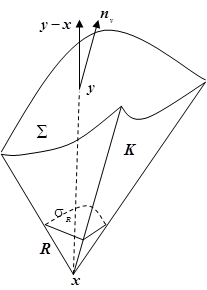
\includegraphics[]{{../img/24-1}.png}
\end{figure}

\begin{definition}
	\textit{Тілесним кутом спостереження} поверхні $\Sigma$ з деякої точки $x \in \RR^3$ будемо називати величину
	\begin{equation}
		\omega(x, \Sigma) = \frac{\sigma_R}{R^2}.
	\end{equation}
\end{definition}

Остання величина, очевидно, не залежить від радіусу сфери $R$ і тому представляє міру тілесного кута. \medskip

У випадку, коли поверхня $\Sigma$ є такою, що величина $\cos(\vec n_y, y - x)$ змінює свій знак в залежності від положення точки $y$, для визначення тілесного кута спостереження такої поверхні, вона розбивається на окремі частини $\Sigma = \bigsqcup_i \Sigma_i$, на кожній з яких $\sign(\cos(\vec n_y, y - x)) = \const$, $y \in \Sigma_i$. \medskip

Таким чином
\begin{equation}
	\omega(x, \Sigma) = \Sum_i \omega(x, \Sigma_i) \cdot \left. \sign(\cos(\vec n_y, y - x)) \right|_{y \in \Sigma_i}.
\end{equation}

\begin{lemma}
	Для будь-якої кусково-гладкої поверхні $\Sigma$, кут спостереження цієї поверхні визначається за формулою
	\begin{equation}
		\omega(x, R) = -\Iiint_\Sigma \frac{\partial}{\partial \vec n_y} \frac{1}{|x - y|} \diff S_y.
	\end{equation}
\end{lemma}

\begin{theorem}[про обмеженість кута спостереження для скінченої поверхні Ляпунова]
	\label{th:4.8.5}
	Якщо $\Sigma$ --- скінченна поверхня Ляпунова, то існує така постійна $C_0$, що
	\begin{equation}
		\label{eq:4.8.61}
		\Iiint_\Sigma \left| \frac{\partial}{\partial \vec n_y} \frac{1}{|x - y|} \right| \diff S_y \le C_0.
	\end{equation}
\end{theorem}

\end{document}